
%(BEGIN_QUESTION)
% Copyright 2006, Tony R. Kuphaldt, released under the Creative Commons Attribution License (v 1.0)
% This means you may do almost anything with this work of mine, so long as you give me proper credit

When using a thermocouple calibrator (simulator), where you simply set it to simulate a thermocouple at a specified temperature, is it important to use the correct thermocouple or extension wire to connect the calibrator with the transmitter, or is the wire type irrelevant?

$$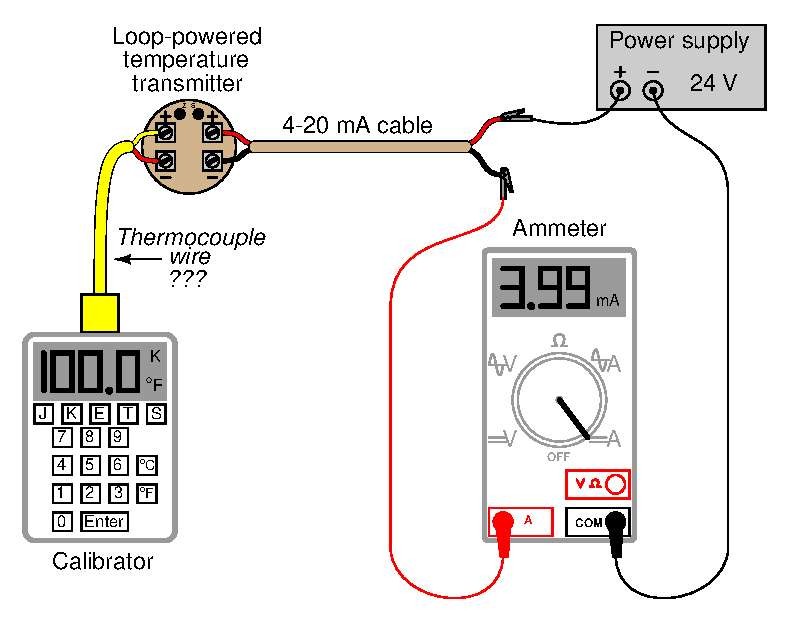
\includegraphics[width=15.5cm]{i00396x01.eps}$$

Be sure to explain your answer, based on the presence of dissimilar-metal junctions and junction-compensation circuitry in both the calibrator and transmitter.

\underbar{file i00396}
%(END_QUESTION)





%(BEGIN_ANSWER)

Ideally, we may use any type of connection wire we wish so long as both the calibrator and the transmitter are at the exact same temperature!  If the temperatures are not the same, we must be sure to use the correct type of thermocouple wire (or extension wire) to connect the calibrator to the instrument.

%(END_ANSWER)





%(BEGIN_NOTES)

Having said this, it is still recommended to use the same type wire as the thermocouple, just in case the two instruments' connection jacks have not equalized in temperature.

It is also recommended to let the calibrator temperature equalize with the transmitter, to eliminate the potential problems of having two sets of reference junctions (and compensating circuits) doing different things at different temperatures.

%INDEX% Measurement, temperature: thermocouple calibrator (simulator)

%(END_NOTES)


